% G02/G03 arc syntax: sign of R (left) and centre offsets I, J (right)
\documentclass[dvisvgm,tikz,border=4pt]{standalone}
% Shared preamble for the TikZ figures in images-1/src (compiled by build.sh)
\usepackage{helvet}
\renewcommand\familydefault{\sfdefault}
\usepackage{amsmath, amssymb}
\usetikzlibrary{arrows.meta, calc, decorations.pathreplacing, patterns, positioning, shapes.geometric, 3d, perspective, fit, backgrounds}
% palette shared with slides.scss and the Graphviz diagrams
\definecolor{dmred}{HTML}{880000}
\definecolor{dmblue}{HTML}{000088}
\definecolor{dmgreen}{HTML}{008800}
\definecolor{dmorange}{HTML}{E08A1E}
\definecolor{ink}{HTML}{333333}
\definecolor{fillblue}{HTML}{E8E8F8}
\definecolor{fillred}{HTML}{F3EAEA}
\definecolor{fillgreen}{HTML}{E8F4E8}
\definecolor{fillorange}{HTML}{FDF0DC}
\definecolor{steel}{HTML}{C9D3DC}
\definecolor{steeldk}{HTML}{8FA3B5}
\definecolor{metal}{HTML}{D9D9D9}
\definecolor{metaldk}{HTML}{A6A6A6}
\tikzset{
  >={Stealth[length=7pt]},
  every picture/.style={line cap=round, line join=round, font=\large},
  proj/.style={gray, dashed, thin},
  dim/.style={<->, >={Stealth[length=5pt]}, thin},
  ext/.style={very thin, gray},
  callout/.style={gray!70!black, thin},
  % datum (origin) symbol
  % pics use absolute sizes so they look the same in mm-scaled drawings
  datum/.pic={
    \fill[white] (0,0) circle (0.22cm);
    \fill[black] (0,0) -- ++(0.22cm,0) arc[start angle=0, end angle=-90, radius=0.22cm] -- cycle;
    \fill[black] (0,0) -- ++(-0.22cm,0) arc[start angle=180, end angle=90, radius=0.22cm] -- cycle;
    \draw[thick] (0,0) circle (0.22cm);
  },
  % reference symbols (absolute sizes): origins have a double circle with a filled quadrant
  wporigin/.pic={
    \draw[thick, fill=white] (0,0) circle (0.3cm);
    \fill[black] (0,0) -- (0.18cm,0) arc[start angle=0, end angle=-90, radius=0.18cm] -- cycle;
    \draw[thick] (0,0) circle (0.18cm);
    \draw (-0.3cm,0) -- (0.3cm,0) (0,-0.3cm) -- (0,0.3cm);
  },
  machorigin/.pic={
    \draw[thick, fill=white] (0,0) circle (0.3cm);
    \fill[black] (0,0) -- (-0.18cm,0) arc[start angle=180, end angle=90, radius=0.18cm] -- cycle;
    \draw[thick] (0,0) circle (0.18cm);
    \draw (-0.3cm,0) -- (0.3cm,0) (0,-0.3cm) -- (0,0.3cm);
  },
  supportpt/.pic={
    \draw[thick, fill=white] (0,0) circle (0.15cm);
    \draw (-0.15cm,0) -- (0.15cm,0) (0,-0.15cm) -- (0,0.15cm);
  },
  regpt/.pic={
    \draw[thick, fill=white] (0,0) circle (0.24cm);
    \draw[thick] (0,0) circle (0.15cm);
    \draw (-0.15cm,0) -- (0.15cm,0) (0,-0.15cm) -- (0,0.15cm);
  },
  % support / registration point (generic)
  target/.pic={
    \draw[thick, fill=white] (0,0) circle (0.12cm);
    \draw (-0.2cm,0) -- (0.2cm,0) (0,-0.2cm) -- (0,0.2cm);
  },
}

\begin{document}
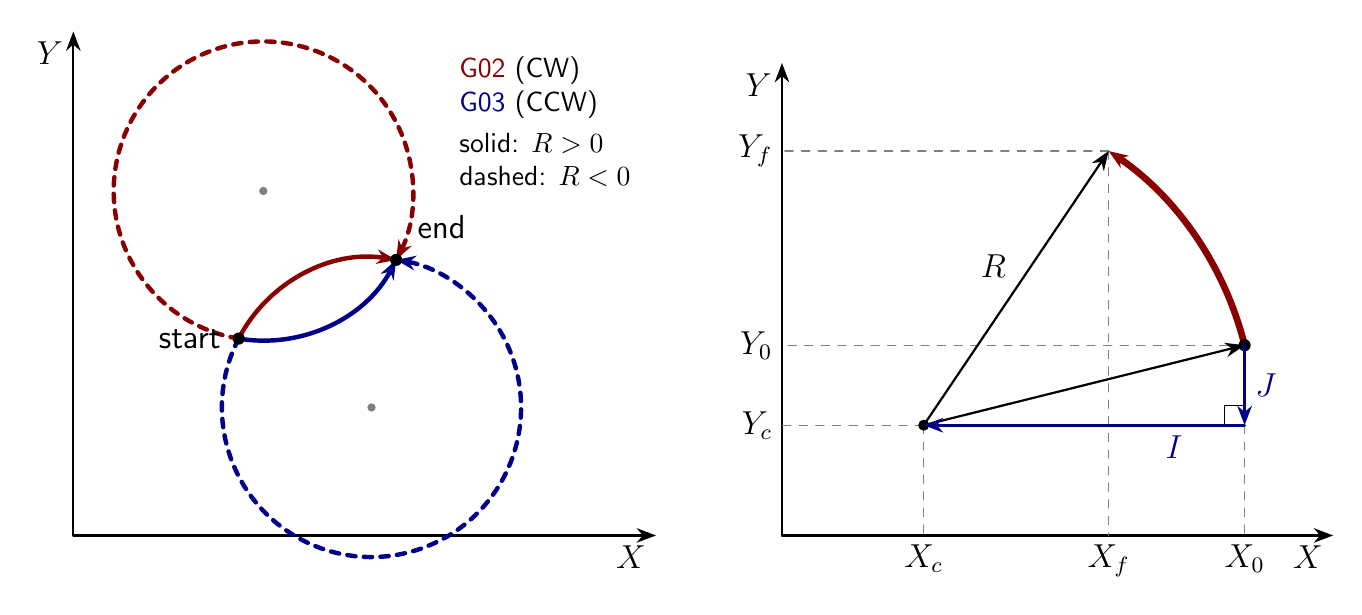
\begin{tikzpicture}
  % ---------- left: the same end points, four possible arcs
  \begin{scope}
    \draw[->, thick] (0,0) -- (7.4,0) node[below left] {$X$};
    \draw[->, thick] (0,0) -- (0,6.4) node[below left] {$Y$};
    \coordinate (A) at (2.1,2.5);   % start
    \coordinate (B) at (4.1,3.5);   % end
    \def\r{1.9}
    % centres on the perpendicular bisector of AB
    \path let \p1=($(B)-(A)$), \n1={veclen(\x1,\y1)/2}, \n2={sqrt((\r cm)^2-(\n1)^2)}, \n3={atan2(\y1,\x1)} in
      coordinate (M) at ($(A)!0.5!(B)$)
      coordinate (Cl) at ($(M)+(\n3+90:\n2)$)
      coordinate (Cr) at ($(M)+(\n3-90:\n2)$);
    % CCW (G03): short arc about the centre left of AB, long arc about the right one
    % CW  (G02): short arc about the centre right of AB, long arc about the left one
    \foreach \C/\col/\dir/\sty in {Cl/dmblue/1/solid, Cr/dmblue/1/dashed, Cr/dmred/-1/solid, Cl/dmred/-1/dashed}{
      \draw[\col, \sty, line width=1.6pt, ->] let \p1=($(A)-(\C)$), \p2=($(B)-(\C)$),
          \n1={atan2(\y1,\x1)}, \n2={atan2(\y2,\x2)},
          \n3={\n1 + \dir*mod(\dir*(\n2-\n1)+720, 360)} in
        (A) arc[start angle=\n1, end angle=\n3, radius=\r];
    }
    \fill (A) circle (2.2pt) node[left=3pt] {start};
    \fill (B) circle (2.2pt) node[above right=6pt] {end};
    \fill[gray] (Cl) circle (1.5pt) (Cr) circle (1.5pt);
    \node[font=\normalsize, align=left, anchor=north east] at (7.2,6.2)
      {\textcolor{dmred}{G02} (CW)\\ \textcolor{dmblue}{G03} (CCW)\\[3pt] solid: $R>0$\\ dashed: $R<0$};
  \end{scope}
  % ---------- right: I, J offsets from the start point to the centre
  \begin{scope}[xshift=9cm]
    \draw[->, thick] (0,0) -- (7,0) node[below left] {$X$};
    \draw[->, thick] (0,0) -- (0,6) node[below left] {$Y$};
    \coordinate (C) at (1.8,1.4);
    \def\R{4.2}\def\tz{14}\def\dt{42}
    \coordinate (P0) at ($(C)+(\tz:\R)$);
    \coordinate (Pf) at ($(C)+(\tz+\dt:\R)$);
    \draw[proj] (C) -- (C|-0,0) node[below, black] {$X_c$};
    \draw[proj] (Pf) -- (Pf|-0,0) node[below, black] {$X_f$};
    \draw[proj] (P0|-C) -- (P0|-0,0) node[below, black] {$X_0$};
    \draw[proj] (C) -- (0,0|-C) node[left, black] {$Y_c$};
    \draw[proj] (Pf) -- (0,0|-Pf) node[left, black] {$Y_f$};
    \draw[proj] (P0) -- (0,0|-P0) node[left, black] {$Y_0$};
    \draw[->, thick] (C) -- (P0);
    \draw[->, thick] (C) -- node[above left] {$R$} (Pf);
    \draw[->, line width=2.4pt, dmred] (P0) arc[start angle=\tz, end angle=\tz+\dt, radius=\R];
    \fill (P0) circle (2.2pt) (C) circle (2pt);
    % J then I: from the start point to the centre, closing a right triangle with the radius
    \coordinate (K) at (P0|-C);
    \draw[thin] ($(K)+(-0.25,0)$) -- ++(0,0.25) -- ++(0.25,0);
    \draw[->, very thick, dmblue] (P0) -- node[right] {$J$} (K);
    \draw[->, very thick, dmblue] (K) -- node[below, pos=0.22] {$I$} (C);
  \end{scope}
\end{tikzpicture}
\end{document}
